\chapter{Association rules \& sequential patterns}
%
\section{Association rules}
Deze \emph{machine learning}-techniek is ontstaan dankzij supermarkten, welke grote datasets hadden met aankopen van verschillende klanten. Voor deze winkels is het interessant om patronen te vinden in deze aankopen, waar ze dan kunnen op inspelen met commerci\"ele aanbiedingen. Het doel is om \emph{association rules} te vinden tussen verschillende aankopen. Een voorbeeld is dat \textbf{als} een klant wijn koopt, \textbf{dan} zal de klant ook kaas zal kopen. Dit noteert men formeel door:

\begin{equation}
wijn \Rightarrow kaas
\end{equation}

Ieder product dat de klant aankoopt wordt een item $i$ genoemd, welke in de ongeordende set van alle aangeboden items $I$ zit:

\begin{equation}
I = \{i_1, i_2, i_3, .., i_m\}
\end{equation}

Daarnaast worden alle transacties (afrekenen aan de kassa) bijgehouden, waarbij elke transactie $t$ bestaat uit een subset van de verzameling van items $I$.

\begin{equation}
T = \{t_1, t_2, t_3, .., t_n \mid t \subseteq I \}
\end{equation}

Een \emph{association rule} is dus een regel tussen twee subsets $X$ en $Y$ van de itemset $I$, welke---uiteraard---verschillende items bevatten. Want niemand is ge\"interesseerd in het feit dat als klanten brood kopen, dan ook brood kopen. 

\begin{equation}
X \Rightarrow Y \textrm{ met } X, Y \subseteq I \textrm{ en } X \cap Y = \emptyset
\end{equation}
%
\subsection{Support en confidence}
Om nuttige regels te kunnen onderscheiden van alle mogelijke regels, dienen deze regels een minimale drempelwaarde te halen voor bepaalde parameters. Twee veelgebruikte parameters zijn \emph{support} en \emph{confidence}. 
%
\paragraph{Support}
Deze parameter geeft aan hoe vaak een itemset $A$ voorkomt in de dataset van transacties $T$. 

\begin{equation}
\supp(X \cup Y) = \frac{|X \cup Y|}{|T|}
\end{equation}

Om een \emph{association rule} te kunnen opstellen, dient een frequente itemset gevonden te worden. Dit is een itemset $X \cup Y$ welke een bepaalde drempelwaarde overschrijdt. 
%
\paragraph{Confidence}
Deze parameter is een indicatie van hoe vaak een regel $ X \Rightarrow Y $ waar blijkt te zijn. Dus hoe vaak alle items $X \cup Y $ voorkomen ten opzichte van hoe vaak $X$ in totaal voorkomt. 

\begin{equation}
\conf(X \Rightarrow Y) = \frac{\supp(X \cup Y)}{\supp(X)}= \frac{|X \cup Y|}{|X|}
\end{equation}

\paragraph{Voorbeeld} Bij wijze van oefening beschouwen we de volgende set met zeven transacties, waarop we de regel $\{eieren, kleding\} \Rightarrow \{melk\}$ toetsen.

\begin{table}[h]
\centering
\caption{Set van transacties $T$}
\label{tabel:7-transacties}
\begin{tabular}{l}
$t_1 = \{wijn, eieren, melk\}$ \\
$t_2 = \{wijn, kaas\}$ \\
$t_3 = \{kaas, laarzen\}$ \\
$t_4 = \{wijn, eieren, kaas\}$ \\
$t_5 = \{wijn, eieren, kleding, kaas, melk\}$ \\
$t_6 = \{eieren, kleding, melk\}$ \\
$t_7 = \{eieren, kleding, melk\}$
       
\end{tabular}
\end{table}

De set $\{eieren, kleding, melk\}$ komt 3 maal voor in de totale set van 7 transacties, dus de \emph{support} is:

\begin{equation}
\supp(\{eieren, kleding, melk\}) = \frac{3}{7}
\end{equation}

in tabel \ref{tabel:7-transacties} is ook te zien dat de set $\{eieren, kleding\}$ driemaal voorkomt. Daarnaast is de set $\{melk\}$ ook altijd aanwezig is indien de voorgaande set een subset van een transactie $t$ is, de gecombineerde set komt dus ook drie keer voor. In dit geval is de \emph{confidence} dus:

\begin{equation}
\conf(\{eieren, kleding\} \Rightarrow \{melk\}) = \frac{3}{3}
\end{equation}
%
\subsection{Mining algoritmes}
Om in een dataset \emph{association rules} te vinden, bestaan er veel algoritmes. Deze zouden, gegeven een minimum \emph{support} en minimum \emph{confidence}, uit dezelfde dataset eenzelfde set regels moeten extraheren. Op vlak van effici\"entie en geheugengebruik kunnen er uiteraard wel verschillen zijn. 

Een na\"ieve strategie om alle regels te vinden in een bepaalde dataset met $m$ items, is om alle regels te genereren en te toetsen aan de vooropgestelde minima. Uiteraard is dit ---zeker met grote itemsets $m >> 1$---niet altijd realiseerbaar. Het aantal regels (inclusief deze die de vooropgestelde drempelwaarden niet halen) is namelijk:

\begin{equation}
|R| = 3^m - 2^{m + 1} + 1
\end{equation}

Het Apriori algoritme is in 1994 bedacht, met als doel het vinden van alle \emph{association rules} in een transactionele dataset op basis van frequente itemsets. Men onderscheidt twee stappen:

\begin{enumerate}
\item Vind alle frequente itemsets met een minimale \emph{support} tot en met een $k$-itemset, waarbij $k$ het aantal items voorstelt.
\item Gebruik deze frequente itemsets om \emph{association rules} te genereren, welke de boven de minimale \emph{confidence} scoren.
\end{enumerate}

Om de eerste stap te realiseren, is het algoritme gebasseerd op de \emph{downward closure}-eigenschap: iedere subset van van een frequente itemset is ook een frequente itemset. 

\begin{figure}
\centering
\caption{Itemset $\{1,2,3\}$ is een frequente itemset; als gevolg van de \emph{downward closure}-eigenschap zijn de subsets ook frequente itemsets.}
\label{figure:downward}
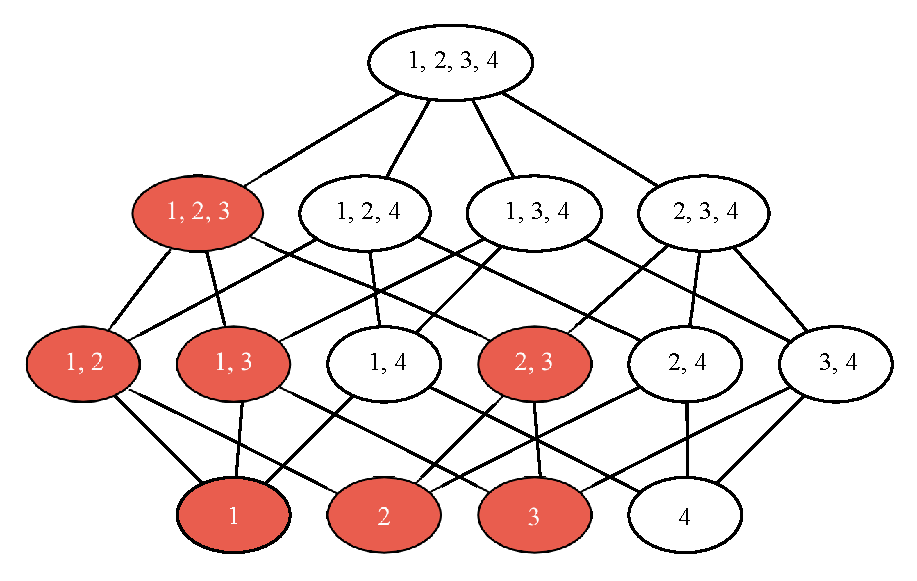
\includegraphics[]{res/downward.eps}
\end{figure}

%%%%%%%%%%%%%%%%%%
% Indien dit gekopieerd wordt, zie: https://en.wikibooks.org/wiki/LaTeX/Algorithms
%%%%%%%%%%%%%%%%%%
\begin{algorithm}
\caption{Pseudocode van Apriori, waarbij de frequente itemsets ontdekt worden.}
\label{algo:apriori}
\begin{algorithmic}
\Require T: Transactionset
\Function{apriori}{T}
    \State $C_1 \gets initialPass(T)$
    \Comment{Generating frequent 1-itemsets}
    \State $F_1 \gets \{f \mid f \in C_1 \wedge minsup \leq \frac{|f|}{|T|} \}$
    \State $k\gets 2$
    \While {$F_{k-1} \neq \emptyset$}
        \State $C_k \gets candidateGen(F_{k-1})$
        \For {$t \in T$} 
        \Comment{Iterate over all transactions}
            \For {$c \in C_{k} $}
                \If {$c \subseteq t$}
                    \State $|c|\gets |c| + 1$
                    \Comment{Increase count of candidate c}
                \EndIf
            \EndFor
        \EndFor
        \State $F_k \gets \{c\mid minsup \leq \frac{|c|}{|T|} \}$
        \State $k \gets k + 1$
    \EndWhile
    \State \Return $F \gets \cup_k F_k$ 
\EndFunction
\end{algorithmic}
\end{algorithm}

\newpage
Apriori past deze eigenschap toe door eerst de 1-item frequente itemsets te zoeken; door permutatie onstaan dan kandidaat-2-itemsets. Deze worden getest of ze voldoen aan de minimale \emph{support}. Indien dit het geval is, worden ze toegevoegd aan de frequente 2-itemset. Dit proces wordt iteratief herhaald tot alle frequente k-itemsets gevonden zijn.

Het genereren van de kandidaten wordt beschreven in algoritme \ref{algo:candidateGen}; de functie genereert een superset van frequente k-itemsets $ C_k \supseteq F_k$ op basis van de frequente itemsets $F_{k-1}$. Dit gebeurt in in twee stappen:

\begin{enumerate}
\item \textbf{Join}: Alle mogelijke kandidaat-k-itemsets $C_k$ worden gegenereerd op basis van $F_{k-1}$.
\item \textbf{Prune}: Kandidaten welke---door de \emph{downward closure property}---niet frequent kunnen zijn worden verwijderend uit $C_k$.
\end{enumerate}

Om de \emph{join}-stap te voltooien, worden kandidaat-k-itemsets beschreven volgens:

\begin{equation}
C_k \gets \{a \cup \{b\} \mid a \in F_{k-1} \wedge b \notin a \}
\end{equation}

De itemset $a$ is dus een element van de set van frequente-k-1-itemset, wat maakt dat $a$ zelf een frequente-k-1-itemset is. Bij deze itemset $a$ wordt een item $b$ toegevoegd, wat niet voorkomt in de itemset $a$. Hierdoor is een k-itemset ontstaan.

\begin{equation}
\{s \mid s \subset c \wedge |s| = k - 1\}
\end{equation}

De \emph{prune}-stap verwijdert alle subsets $s \subset c$ uit de kandidaten $c \in C_k$ die niet voorkwomen in de frequente itemset $F_{k-1}$. De subset $s$ moet voor deze reden $k-1$ items bevatten.

%%%%%%%%%%%%%%%%%%
% Indien dit gekopieerd wordt, zie: https://en.wikibooks.org/wiki/LaTeX/Algorithms
%%%%%%%%%%%%%%%%%%
\begin{algorithm}
\caption{Pseudocode om kandidaten te genereren uit frequente k-1-itemsets.}
\label{algo:candidateGen}
\begin{algorithmic} 
\Require $F_{k-1}$: Frequent k-1-itemset
\Function{candidateGen}{$F_{k-1}$}
    \State $C_k \gets \emptyset$
    \Comment{Starting with an empty set}
    \For {$C_k \gets \{a \cup \{b\} \mid a \subset F_{k-1} \wedge b \notin a \}$}
    	\Comment{Join}
        \For {$\{s \mid s \subset c \wedge |s| = k - 1\}$} 
        	\If {$s \notin F_{k-1}$}
            	\State $C_k \gets C_k - c$ 
                \Comment{Prune}
            \EndIf
        \EndFor
    \EndFor
    \State \Return $C_k$ 
\EndFunction
\end{algorithmic}
\end{algorithm}
%
Algoritme \ref{algo:apriori} is dus in staat alle frequente itemsets met een minimale \emph{support} $minsup$ te ontdekken, hieruit kunnen dan \emph{association rules} gedestilleerd worden. Dit gebeurt door voor iedere frequente itemset $F_k \in F$ iteratief iedere strikte subset $E \subset F_k$ te toetsen aan de minimale \emph{confidence} $minconf$.
%
%%%%%%%%%%%%%%%%%%
% Indien dit gekopieerd wordt, zie: https://en.wikibooks.org/wiki/LaTeX/Algorithms
%%%%%%%%%%%%%%%%%%
\begin{algorithm}
\caption{Pseudocode om \emph{asssociation rules} uit frequente itemsets te genereren.}
\label{algo:step_2}
\begin{algorithmic} 
\Require $F$: Set of frequent itemsets
\Function{rulesGen}{$F$}
    \For {$F_k \in F$}
        \For {$\{E \subset F_k| E \neq \emptyset \wedge E \neq F_k \}$} 
        	\If {$\conf\left(E \Rightarrow E \cap F_k \right) \geq minconf$}
            	\State Assocation rule $E \Rightarrow E \cap F_k$ found
            \EndIf
        \EndFor
    \EndFor
\EndFunction
\end{algorithmic}
\end{algorithm}
%
\subsection{Zeldzame itemprobleem}
In bepaalde datasets komen bepaalde items significant meer voor dan andere items. In het voorbeeld van de supermarkt zien we bijvoorbeeld terug in de wekelijkse aankoop van brood en de---hopelijk---eenmalige aankoop van een broodrooster. Het probleem is dus dat de minimaal benodigde \emph{support} voor ieder item hetzelfde is, onafhankelijk van de frequentie van dat item. De keuze van deze drempelwaarde heeft dus een twee gevolgen:

\begin{itemize}
\item \textbf{Minimale \emph{support} is hoog}: \emph{Association rules} met \emph{rare items} zullen niet gevonden worden.
\item \textbf{Minimale \emph{support} is laag}: Frequente items zullen met elkaar gecombineerd worden, wat ook minder betekenisvolle regels tot gevolg heeft. 
\end{itemize}

Door individuele items een \emph{minimum item support} MIS toe te kennen, wat we noteren als $\MIS\left(i\right)$, kan dit probleem opgelost worden. De \emph{support} dient dan groter te zijn dan de minimale MIS van itemset $X \cup Y = \{i_1, i_2, ..., i_r\} \textrm{ met } i_j \in I$.

\begin{equation}
\supp(X \cup Y) \geq \min\left(\MIS(i_1), \MIS(i_2), ..., \MIS(i_r) \right)
\end{equation}

Om te verhinderen dat frequente items samen met \emph{rare items} voorkomen, mag het verschil tussen de grootste en kleinste MIS niet groter zijn dan een bepaalde drempelwaarde. Dit wordt de \emph{support difference constraint} $\phi$ genoemd. 

\begin{equation}
\phi \geq \max_{i\in X \cup Y}\left(\supp(i) - \min_{i\in X \cup Y}\left(\supp(i)\right)\right)
\end{equation}

Wat vereenvoudigd kan worden tot:

\begin{equation}
\phi \geq \max_{i\in X \cup Y}\left(\supp(i)\right) - \min_{i\in X \cup Y}\left(\supp(i)\right)
\end{equation}

Door de introductie van \emph{minimum item supports} is de \emph{downward closure}-eigenschap niet meer geldig\cite{Liu1999MiningSupports}. Een alternatief hiervoor is \emph{sorted closure}; waarbij items gesorteerd worden volgens hun MIS. Dit valt echter buiten de scope van deze cursus.
%
\subsection{Class association rules}
Bij \emph{association mining} kunnen items voorkomen als een conditie $i \in X$ of als een consequentie $i \in Y$. Indien men echter enkel ge\"interesseerd is in de regels die een bepaalde consequentie opleveren, dan willen we alle \emph{class association rules} (CAR) met een klasse $y$ van de set van klasse-labels $Y$ vinden. Formeel wordt dit:

\begin{equation}
X \Rightarrow y \textrm{ met } X \subseteq I \textrm{ en } y \in Y
\end{equation}

Aangezien de klasse-labels al gekend zijn, is het vinden van frequente k-itemsets voldoende om de regels te genereren. Dit betekent dus dat Apriori aangepast kan worden voor CAR. 

Daarnaast is het ook nuttig om op te merken dat de gekende definities voor de \emph{support} en \emph{confidence} hetzelfde blijven.
%
\newpage
\begin{table}
\centering
\caption{Set van transacties $T$.}
\label{tabel:7-transacties}
\begin{tabular}{c|c|c}
\textbf{Doc} & \textbf{Dataset} & \textbf{Klasse} \\
1 & $\{student, leerkracht, school\}$ & $onderwijs$ \\
2 & $\{student, school\}$ & $onderwijs$ \\
3 & $\{leerkracht, school, stad, wedstrijd\}$ & $onderwijs$\\
4 & $\{basketball, lopen\}$ & $sport$ \\
5 & $\{basketball, speler, toeschouwer\}$ & $sport$\\
6 & $\{basketball, coach, wedstrijd, team\}$ & $sport$\\
7 & $\{basketball, team, stad, wedstrijd\}$ & $sport$
\end{tabular}
\end{table}
%
\paragraph{Voorbeeld}
Stel $minsup = 20\%$ en $minconf = 60\%$. We beschouwen de dataset in tabel \ref{tabel:7-transacties}, welke bestaat uit enkele frequente woorden van documenten die geclassificeerd zijn als \emph{sport} of \emph{onderwijs}.

\begin{table}
\centering
\caption{Ontdekte regels uit de transacties opgesomd in tabel \ref{tabel:7-transacties}.}
\label{tabel:regels-7-transacties}
\begin{tabular}{c|c|c}
\textbf{Regel} & \textbf{supp} & \textbf{conf} \\
$\{student, school\} \Rightarrow onderwijs$ & $\dfrac{2}{7}=29\%$ & $\dfrac{2}{2}=100\%$\\[10pt]
$\{basketball\} \Rightarrow sport$ & $\dfrac{4}{7}=57\%$ & $\dfrac{4}{4}=100\%$\\[10pt]
$\{wedstrijd\} \Rightarrow sport$ & $\dfrac{2}{7}=29\%$ & $\dfrac{2}{3}=67\%$ \\[10pt]
$\{team\} \Rightarrow sport$ & $\dfrac{2}{7}=29\%$ & $\dfrac{2}{2}=100\%$ \\[10pt]
$\{basketball, wedstrijd\} \Rightarrow sport$ & $\dfrac{2}{7}=29\%$ & $\dfrac{2}{2}=100\%$\\[10pt]
$\{basketball, team\} \Rightarrow sport$ & $\dfrac{2}{7}=29\%$ & $\dfrac{2}{2}=100\%$\\[10pt]
$\{team, wedstrijd\} \Rightarrow sport$ & $\dfrac{2}{7}=29\%$ & $\dfrac{2}{2}=100\%$\\[10pt]
$\{basketball, wedstrijd, team\} \Rightarrow sport$ & $\dfrac{2}{7}=29\%$ & $\dfrac{2}{2}=100\%$\\

\end{tabular}
\end{table}

%
\section{Sequenti\"ele patronen}
Een limitatie van voorgaande \emph{association rules} is dat er geen rekening gehouden wordt met de volgorde van transacties. Het kan echter wel nuttig zijn om deze volgorde in beschouwing te nemen, wat leidt tot sequenties. Men defini\"eert een sequentie $s$ als een \textbf{geordende} lijst van itemsets $a_i$. Een k-sequentie is een sequentie van k itemsets; wat gelijkaardig is aan k-itemsets.

\begin{equation}
s = \langle a_1, a_2, a_3, ..., a_r \mid a \subseteq I  \rangle
\end{equation}

\paragraph{sub- en supersequenties}
Indien we twee sequenties $s_1 = \langle a_1, ..., a_r \rangle
$ en $s_2 = \langle b_1, ..., b_v \rangle$ beschouwen, dan kunnen we stellen dat sequentie $s_1$ een \emph{subsequentie} is van sequentie $s_2$ als iedere itemset ook een deelverzameling is. 
\begin{equation}
s_1 \subseteq s_2 \iff \{a_i \subseteq b_i \mid \{i \in \langle\mathds{Z}^{+}\rangle \mid i \leq r \} \} 
\end{equation}

\subsection{Mining algoritmes}
Om sequenties te \emph{minen}, kan het \emph{Generalized Sequential Pattern} of kortweg GSP-algoritme gebruikt worden. Dit algoritme lijkt zeer sterk op Apriori---wat bij algoritme \ref{algo:apriori} is besproken. Wat wel verschilt is de generatie van kandidaten. De twee stappen (\emph{join} en \emph{prune}) van Apriori komen ook wel weer terug:

\begin{enumerate}
\item \textbf{Join}: Alle mogelijke kandidaat-k-sequenties worden gegenereerd door $F_{k-1}$ te \emph{joinen} met $F_{k-1}$. De volledige sequentie $s_1$ \emph{joint} de volledige sequentie $s_2$ als de subsequentie van $s_1$ zonder het eerste item gelijk is aan de subsequentie van $s_2$ zonder het laatste item. 

Afhankelijk of het laatste element van $s_2$ een aparte set vormt, zijn er twee gevallen: 
\begin{enumerate}
\item Het item vormt een aparte set op het einde van $s_1$ als het ook een aparte set vormde in $s_2$.
\item Het item wordt aan het laatste element van $s_1$ toegevoegd indien het geen aparte set vormde in $s_2$.
\end{enumerate}

Het \emph{joinen} van $F_1$ met $F_1$ is ook bijzonder, aangezien er hier nog geen itemsets zijn ($k=1$). Dus wordt het item van $s_2$ zowel als itemset als apart element toegevoegd.
\item \textbf{Prune}: Kandidaten waarbij een van de k-1-subsequenties niet frequent is, worden verwijderd.
\end{enumerate}

\paragraph{Voorbeeld} In tabel \ref{tabel:candidates-3-sequences} wordt de generatie van kandidaten uitgewerkt. Indien we we het algoritme overlopen en stellen dat $s_1 = \langle \{1,2\}\{4\}\rangle $, dan is de subsequentie zonder het eerste item $\langle \{2\}\{4\}\rangle $. Dit komt overeen met de laatste twee frequente-3-sequenties. Deze worden dan gecombineerd, rekening houdende met de bovengestelde voorwaarde. 

\begin{table}
\centering
\caption{Kandidaten uit frequente-3-sequenties.}
\label{tabel:candidates-3-sequences}
\begin{tabular}{c|c|c}
\textbf{Frequente-3-}& \multicolumn{2}{c}{\textbf{Kandidaat-4-sequenties}} \\
\textbf{sequenties} & \textbf{Na \emph{join}} & \textbf{Na \emph{prune}} \\
$ \langle \{1,2\}\{4\}\rangle $ & $ \langle \{1,2\}\{4,5\}\rangle $ & $\langle \{1,2\}\{4,5\}\rangle $ \\ 
$ \langle \{1,2\}\{5\}\rangle $ & $ \langle \{1,2\}\{4\}\{6\}\rangle $ & \\ 
$ \langle \{1\}\{4,5\}\rangle $ &  & \\ 
$ \langle \{1,4\}\{6\}\rangle $ &  & \\ 
$ \langle \{2\}\{4,5\}\rangle $ &  & \\ 
$\langle\{2\}\{4\}\{6\}\rangle$ &  & \\ 


\end{tabular}
\end{table}